\renewcommand{\theequation}{\theenumi}
\begin{enumerate}[label=\arabic*.,ref=\thesubsection.\theenumi]
\numberwithin{equation}{enumi}

	\item If the expression \\
	$\frac{[\sin(\frac{x}{2})+\cos(\frac{x}{2})+i\tan(x)]}{[1+ 2 i \sin{\frac{x}{2}}]}$
    is real, then the set of all possible values of x  is $.........$
    \item For any two complex numbers $z_1,z_2$ and any two real number a and b. 
    $\abs{az_1-bz_2}^2 + \abs{bz_1+az_2}^2 =.............$
    \item If a,b,c, are the numbers between 0 and 1 such that the points $z_1=a
    +i,z_2 = 1+bi$ and $z_3=0$ form a equilateral triangle, then $a=.....$ and $b=.............$
    \item ABCD is a rhombus. Its diagonals AC and BD intersect at the point M and satisfy BD = 2AC.If the points D and M represent the complex numbers 1+i and 2-i  respectively.then A represents the complex numbers$.....$ or$.............$
    \item Suppose $Z_1,Z_2,Z_3$ are the vertices of an equilateral triangle inscribed in the circle
     $\abs Z = 2$. If$Z_1 = 1+i\sqrt{3}$ then $Z_2 =............Z_3$=.....
    \item The values of the expression
    $1\bullet(2-\omega)(2-\omega)^2+2.(3-\omega)(3-\omega)^2+....(n-1) \bullet(n-\omega)(n-\omega)^2$,
    where $\omega$ is the an imaginary cube root of unity, is $...$
 \item For complex number $z_1 = x_1+iy_1$ and $z_2 = x_2+iy_2$, we write $z_1\cap z_2$, if $x_1 \leq x_2$ and $y_1 \leq y_2$.then for all complex numbers z with $1\cap z$,we have ${{\frac{1-z}{1+z}}}\cap0.$
    \item If the complex numbers $Z_1,Z_2$ and $Z_3$ represent the vertices of an equilateral triangle such that  $\abs{Z_1} = \abs{Z_2} = \abs{Z_3}$ then $Z_1$+$Z_2$+$Z_3 = 0$
    \item If three complex numbers are in A.P. then they lie on a circles in the complex plane.  
    \item The cube roots of unity when represented on Argand  diagram from the vertices of an equilateral triangle.
	\item If the cube roots of unity are 1, $\omega$, $\omega^2$, then the roots of the equation     
	$(x-1)^3+8=0$ are $....$
    \begin{enumerate}
    \item  $-1,1+2\omega,1+2\omega^2$
    \item  -1,$1-2\omega,1-2\omega^2$
    \item  -1,-1,-1
    \item  None of the above
    \end{enumerate}
    \item The smallest positive integer for which
     $( {\frac{1+i}{1-i}})^n=1$ is 
     \begin{enumerate}
    \item  n=8
    \item  n=16
    \item  n=12
    \item  None of the above
    \end{enumerate}
    \item The complex numbers z = x+iy which satisfy the equation 
    $\abs{\frac{z-5i}{z+5i}}$ = 1 lie on
    \begin{enumerate}
    \item  the x-axis
    \item  the straight line y=5
    \item   a circle passing through the origin
    \item  None of the above
    \end{enumerate}
    \item if z = $(\frac{\sqrt3}{2}+\frac{i}{2})^5+(\frac{\sqrt3}{2}-\frac{i}{2})^5 $ , then 
     \begin{enumerate}
    \item   Re(z)=0
    \item   Im(z)=0    
    \item  $Re(z) > 0, Im(z) > 0$
    \item  $Re(z)> 0, Im(z)< 0$
    \end{enumerate}
    \item The inequality $\abs{z-4} < \abs{z-2}$ represents the region given by
    \begin{enumerate}
    \item  $Re(z) > 0$
    \item  $Im(z) < 0$
    \item  $Re(z) > 0$
    \item  None of the above
    \end{enumerate}
     \item If z = x+iy and $\omega = \frac{1-iz}{z-i}$, then $\abs{\omega}$ = 1 implies that, in the complex plane,
    \begin{enumerate}
    \item  z lies on the imaginary plane,
    \item  z lies on the real axis
    \item  z lies on the unit circle
    \item  None of these
    \end{enumerate}
    \item The points $z_1, z_2, z_3, z_4$ in the complex plane are the vertices of a parallelogram taken in order if and only if
    \begin{enumerate}
     \item $z_1+z_4=z_2+z_3$
    \item  $z_1+z_3=z_2+z_4$
    \item  $z_1+z_2=z_3+z_4$
    \item None of these
    \end{enumerate}
    \item If a, b, c and u, v, w are complex numbers representing the vertices of two triangle such that 
    $c = (1-r)a + rb$ and $w = (1-r)u + rv$, where r is a complex number, then the two triangles
    \begin{enumerate}
    \item have the same area
    \item  are similar
    \item  are concurrent 
    \item None of these
    \end{enumerate}
    \item If $\omega(\neq1)$ is a cube root of unit and $(1+\omega)^7 = A+B \omega$ then A and B are respectively 
    \begin{enumerate}
    \item 0,1
    \item  1,1
    \item  1,0 
    \item -1,1
    \end{enumerate}
    \item Let z and w be two non zero complex numbers such that $\abs z = \abs w $ and Arg z + Arg $\omega=\pi$ then z equals
    \begin{enumerate}
    \item  $\omega$
    \item  $-\omega$
    \item  $\bar\omega$
    \item  $-\bar\omega$
    \end{enumerate}
    \item Let z and w be two complex numbers such that $\abs{z}\leq$1, $\abs{w}\leq$1 and $\abs{z+iw} = \abs{z-i\bar\omega}$ = 2 then z equals 
   \begin{enumerate} 
    \item 1 or i
    \item  i or -i
    \item  1 or -1
    \item  i or -1
    \end{enumerate}
    \item For positive integer $n_1, n_2$ the value of the expression
    $(1+i)^n_1$ + $(1+i^3)^n_1$ + $(1+i^5)^n_2$ + $(1+i^7)^n_2$, where $i = \sqrt{-1}$ is a real number if and only if
    \begin{enumerate}
    \item  $n_1=n_2+1$
    \item  $n_1=n_2-1$
    \item  $n_1=n_2$
    \item  $n_1 > 0$, $n_2 > 0$
    \end{enumerate}
    \item If i = $\sqrt -1$, then $4+5(-\frac{1}{2}+\frac{i\sqrt3}{2})^{334}+3(-\frac{1}{2}+\frac{i\sqrt3}{2})^{365}$ is equal to 
    \begin{enumerate}
    \item  $1-i\sqrt 3$
    \item  $-1+i\sqrt 3$
    \item  $i\sqrt 3$
    \item  $-i\sqrt 3$
    \end{enumerate}
    \item If arg(z) $< 0$, then arg(-z)-arg(-z)=
    \begin{enumerate}
    \item  $\pi$
    \item  $-\pi$
    \item  $-\pi/2$
    \item  $\pi/2$
    \end{enumerate}
    \item If $z_1, z_2$ and $z_3$ are complex numbers such that 
    $\abs{z_1} =\abs{z_2} = \abs {z_3} = \abs{ \frac{1}{z_1}+\frac{1}{z_2}+\frac{1}{z_3}}$ = 1, 
    then $\abs{ z_1 + z_2 + z_3}$ is 
   \begin{enumerate} 
    \item  equal to 1
    \item  less than 1
    \item  greater than 3
    \item  equal to 3
    \end{enumerate}
    \item Let $z_1$ and $z_2$ be $n^{th}$ roots of unity which subtend a right angle at the origin. Then n must be of the form
    \begin{enumerate}
    \item   $4k+1$
    \item   $4k+2$
    \item   $4k+3$
    \item   $4k$
    \end{enumerate}
    \item  The complex numbers $z_1, z_2$ and $z_3$ satisfying
    $\frac{z_1-z_3}{z_2-z_3} = \frac{1-i\sqrt3}{2}$ are the vertices of a triangle which is
    \begin{enumerate}
    \item   of area zero
    \item   right-angled isosceles
    \item   equilateral
    \item   obtuse-angled isosceles
    \end{enumerate}
    \item For all complex numbers $z_1, z_2$ satisfying $\abs Z_1$ = 12 and $\abs{z_2-3-4i}$ = 5, the minimum value of  $\abs{ z_1-z_2}$ is
    \begin{enumerate}
    \item   0
    \item   2
    \item   7
    \item   17
    \end{enumerate}
    \item If $\abs{z}$ = 1 and $w = \frac{z-1}{z+1}$(where $z \neq -1$), then Re($\omega$) is
    \begin{enumerate}
    \item   0
    \item   $-\frac{1}{\vert z+1\vert ^2}$
    \item   $\frac{z}{z+1}.\frac{1}{\vert z+1\vert ^2}$
    \item   $-\frac{\sqrt 2}{\vert z+1\vert ^2}$
    \end{enumerate}
    \item If $\omega(\neq1)$ be a cube root of unity and $(1+\omega^2)^n$ = $(1+\omega^4)^n$, then the least positive value of n is
    \begin{enumerate}
    \item   2
    \item   3
    \item   5
    \item   6
    \end{enumerate}
    \item The locus of z which lies in shaded region (excluding the boundaries) is best represented by 
        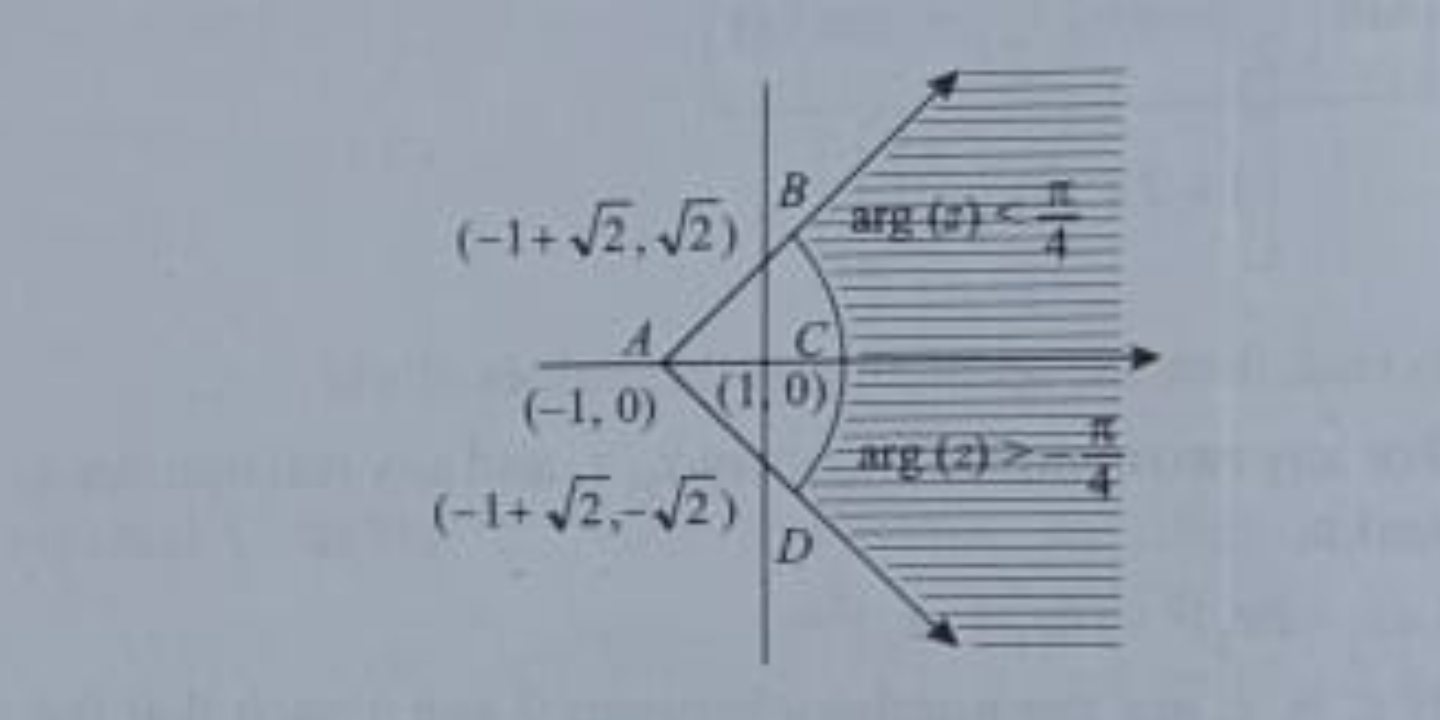
\includegraphics[width=\columnwidth]{./complex/figs/sam.eps}
    \begin{enumerate}
    \item  z:$\abs{ z+1 } > 2$ and $\abs{arg(z+1)} < \pi/4$
    \item   z:$\abs{ z-1} > 2$ and $\abs{ arg(z-1)} < \pi/2$
    \item   z:$\abs{z+1} < 2$ and $\abs{ arg(z+1)} < \pi/4$
    \item   z:$\abs{ z-1} < 2$ and $\abs{ arg(z+1) } < \pi/2$
    \end{enumerate}
    \item a,b,c are integers, not all simultaneously equal and $\omega$ is cube root of unity $(\omega \neq 1)$, then minimum value of $\abs{ a+bw+cw^2} $ is
    \begin{enumerate}
    \item   0
    \item   1
    \item   $\frac{\sqrt3}{2}$
    \item   $\frac{1}{2}$
    \end{enumerate}
    \item Let $w = \frac{-1}{2} + i\frac{\sqrt3}{2}$, then the value of det.
    \\ \myvec{1 & 1 & 1 \\ 1 & -1-\omega^2 & \omega^2 \\ 1 & \omega^2 &\omega^4} is 
    \begin{enumerate}
    \item   $3\omega$
    \item   $3\omega(\omega-1)$
    \item   $3\omega^2$
    \item  $3\omega(1-\omega)$ 
    \end{enumerate}
    \item If $[\frac{w-\bar w z}{1-z}]$ is purely real where $w = \alpha+i\beta$, $\beta \neq 0$ and $z \neq 1$, then the set of the values of z is 
    \begin{enumerate}
    \item   $\{z:\abs z =1\}$
    \item   $\{z:z=\bar z\}$
    \item   $\{z:z\neq1\}$
    \item   $\{z:\abs z=1,z \neq 1\}$
    \end{enumerate}    
    \item A man walks a distance of 3 units from the origin towards the north-east(N 45 degree E) direction. From there, he walks a distance of 4 units toward the north-west(N 45 degree W) direction to each point P. Then the position of P in the Argand plane is
    \begin{enumerate}
    \item   $3e^i\frac{\pi}{4}+4i$ 
    \item   $(3-4i)e^i\frac{\pi}{4}$
    \item   $(4+3i)e^i\frac{\pi}{4}$
    \item   $(3+4i)e^i\frac{\pi}{4}$
    \end{enumerate}
    \item If $\abs z = 1$ and $\abs z \neq 1$ then all the values of $[\frac{z}{1-z^2}]$ lie on 
    \begin{enumerate}
    \item   a line not passing through the origin 
    \item   $\abs z=\sqrt 2$
    \item   the x-axis
    \item   the y-axis    
    \end{enumerate}     
    \item  A particle P starts from point $z_0 = 1+2i$, where $i = \sqrt {-1}$. It moves horizontally away from the origin by 5 units and them vertically away from origin by 3 units to reach a point $z_1$. From $z_1$ is the particle moves $\sqrt{2}$ units in the direction of the vector i+j and then it moves through an angle $\frac{\pi}{2}$ in anticlockwise direction on a circle which centre at origin, to reach a point $z_2$. The point $z_2$ is given by
    \begin{enumerate}  
    \item   $6+7i$ 
    \item   $-7+6i$
    \item   $7+6i$
    \item   $-6+7i$
    \end{enumerate}
    \item Let z = $\cos\theta+i\sin\theta.$ Then the value of $\sum_{m=1}^{15}Im(z^2m-1)$
    at $\theta = 2\degree$ 
    \begin{enumerate}
    \item   $\frac{1}{sin 2 \degree }$ 
    \item   $\frac{1}{3sin 2 \degree }$
    \item   $\frac{1}{2sin 2 \degree }$    
    \item   $\frac{1}{4sin 2 \degree }$
    \end{enumerate}
    \item Let $z = x+iy$ be a complex number where x and y are integers.Then find the area of the rectangle whose vertices are the roots of the equation : $zz^{-3} + \bar z z ^3 = 350$ 
    \begin{enumerate}
    \item 48
    \item 32
    \item 40
    \item 80
    \end{enumerate}    
    \item Let $z$ be a complex numbers such that the imaginary part of $z$ is non-zero and $a = a^2+z+1$ is real. Then a cannot take the value
    \begin{enumerate}        
    \item   $-1$ 
    \item   $\frac{1}{3}$
    \item   $\frac{1}{2}$
    \item   $\frac{3}{4}$
    \end{enumerate}
    \item Let complex numbers $\alpha$ and $\frac{1}{\alpha}$  lie on circles $(x-x_0)^2+(y-y_0)^2\equiv r^2$ and $(x-x_0)^2 (y-y_0)^2\equiv 4r^2$ respectively. If $z_0\equiv x_0+iy_0$ satisfies the equation $2\abs {z_0} ^2 = r^2+2$,then $\abs{\alpha} $=
    \begin{enumerate}
    \item    $\frac{1}{\sqrt 2}$ 
    \item   $\frac{1}{2}$
    \item   $\frac{1}{\sqrt7}$
    \item   $\frac{1}{3}$
    \end{enumerate}
    \item Let S be the set off all complex numbers z satisfying  $\abs z-2+i \geq \sqrt 5$. If the complex numbers $z_0$ is such that ${\abs{\frac{1}{z_0-1}}}$ is the maximum of the set $\{{\vert\frac{1}{z-1}\vert}:z\in S\}$, then the principle argument of $\frac{4-z_0-\bar z_0}{z_0-\bar z_0+2i}$ is 
    \begin{enumerate}
    \item    $\frac{\pi}{4}$ 
    \item   $\frac{3\pi}{4}$
    \item   $\frac{\pi}{2}$
    \item   $\frac{-\pi}{2}$ 
    \end{enumerate}
    \item $z_1 = a+ib$ and $z_2 = c+id$  are complex numbers such that $\abs {z_1} = \abs {z_2}$ = 1 and Re$(z_1 \bar z_2)=0$,then the piar of complex numbers $w_1=a+ic$ and $w_2=b+id$ satisfies 
    \begin{enumerate}
    \item    $\abs w_1 $=1 
    \item   $\abs w_1 $=2
    \item   Re$(w_1 \bar w_2)=0$
    \item   none of these
    \end{enumerate}
    \item Let $z_1$ and $z_2$ be complex numbers such that $z_1\neq z_2$ and  $\abs {z_1} = \abs {z_2} $. If $z_1$ has positive real part and $z_2$ has negative imaginary part,then  $\frac{z_1+z_2}{z_1-z_2}$ may be
    \begin{enumerate}
    \item    zero
    \item   real and positive
    \item   real and negative    
    \item   purely imaginary  
    \item none of these
    \end{enumerate}
    \item If $z_1$ and $z_2$ are two non zero complex numbers such that $\abs{z_1+z_2}$ = $\abs{z_1+ z_2}$, then Arg $z_1$- Arg $z_2$ is equal to
    \begin{enumerate}
    \item    $-\pi$ 
    \item   $\frac{-\pi}{2}$
    \item   $0$    
    \item  $\frac{\pi}{2}$
    \end{enumerate}
    \item The value of $\sum_{k=1}^{6}$ ($\sin\frac{2\pi k}{7}-i\cos\frac{2\pi k}{7}$) is 
    \begin{enumerate}
    \item    $-1$ 
    \item    $0$
    \item   $-i$    
    \item   $i$  
    \item None
    \end{enumerate}
    \item If $\omega$ is an imaginary cube root of unity, then $(1+\omega-\omega^2)^7$ equals 
    \begin{enumerate}
    \item    $128w$ 
    \item    $-128\omega$
    \item   $128\omega^2$    
    \item   $-128\omega^2$
    \end{enumerate}
    \item The value of the sum $\sum_{n=1}^{13}(i^n+i^n+1)$, where $i = \sqrt -1$, equals
    \begin{enumerate}
    \item   $i$ 
    \item   $i-1$
    \item   $-i$    
    \item   $0$
    \end{enumerate}
    \item If $\begin{vmatrix}
    6i &-3i& 1\\ 4&3i&-1 \\20&3&i    \end{vmatrix}$ = x+iy,then 
    \begin{enumerate}
    \item   $x=3,y=2$ 
    \item   $x=1,y=3$
    \item   $x=0,y=3$    
    \item  $x=0,y=0$
    \end{enumerate}
    \item Let $z_1$ and $z_2$ be two distinct complex numbers and let $z=(1-t)z_1+tz_2$ for real some numbers t with $0 < t < 1$.If Arg(w) denotes the principle argument of a non-zero complex number w then 
    \begin{enumerate}
    \item   $\vert z-z_1 \vert+\vert z-z_2 \vert=\vert z_1-z_2 \vert$ 
    \item   $Arg(z-z_1)=Arg(z-z_2)$
    \item   $ \myvec{z-z_1 & \bar z-\bar z_1 \\ z_2-z_1 & \bar z_2-\bar z_1}$         
    \item  $Arg(z-z_1)=Arg(z_2-z_1)$
    \end{enumerate}
    \item Let 
    $w = \frac{\sqrt{3+i}}{2}$ and 
    $P = {w^n:n=1, 2, 3,......}$. Further $H_1 = { z\in C: Rez>\frac{1}{2}}$ and 
    $H_2={ z\in C: Rez<\frac{-1}{2}}$,where c is the set of all complex numbers. 
    If $Z_1 I P C H_1,z_2 I P c H_2$ and O represents the origin. then $\angle z_1 o z_2 =$
    \begin{enumerate}
    \item  $\frac{p}{2}$ 
    \item  $\frac{p}{6}$
    \item  $\frac{2p}{3}$
    \item  $\frac{5p}{6}$
    \end{enumerate}
    \item Let $a,b,c\in R$ and $a^2+b^2\neq = 0$ 
    suppose $S = {Z \in C:Z=\frac{1}{a+ibt},+ \in R,t \neq0}$,where $i = \sqrt-1$.If $z = x+iy$ and $z\in S $,then $\myvec(x,y)$ lies on
    \begin{enumerate}
    \item the circle with radius $\frac{1}{2a}$ and centre $[ \,\frac{1}{2a},0] \,$ for $agr > 0,$	 
    \item  the circle with radius $\frac{-1}{2a}$ and centre $[ \,\frac{-1}{2a},0] \,$ for $a < 0, b\neq 0$
    \item  the x-axis for a $a\neq 0,b=0$
    \item   the x-axis for a $a=0,b\neq 0$
    \end{enumerate}
    \item Let a, b x and y real numbers such that $a-b=1$ and $y\neq 0$. If the complex number $z=x+iy$ satisfies $Im[\frac {az+b}{z+1}] = y$ then which of the following  is(are) possible values(s) of X ?
    \begin{enumerate}
    \item   $-1+\sqrt1-y^2$ 
    \item   $-1-\sqrt1-y^2$
    \item   $1+\sqrt1+y^2$ 
    \item   $1-\sqrt1+y^2$
    \end{enumerate}
    \item For a non-zero complex numbers z let arg(z) denote the principle argument with $-\pi < arg(z)\leq\pi$.Then which of the following statement(s) is(are) $\boldsymbol{FALSE} ?$
    \begin{enumerate}
    \item   $arg(-1-i)=\frac{\pi}{4}$, where $i=\sqrt -1$ 
    \item   the function $ f :R \longrightarrow(-\pi.\pi] \,$, defined by $f(t)=arg(-1+it)$ for all $\in R$, is continues at all points of R, where $i=\sqrt-1$ 
    \item  For any two non-zero complex numbers $z_1$ and $z_2$,
     arg$[ \,\frac{z_1}{z_2}] \,-arg(z_1)+arg(z_2)$ is an integer multiple of $2\pi$
    \item  Foe any three given distinct complex numbers $z_1$, $z_2$ and $z_3$, the locus of the point z satisfying the condition 
         $arg[ \,\frac{(z-z_1)(z_2-z_3)}{(z-z_3)(z_2-z_1)}] \,$=$\pi$,lies on a straight line
    \end{enumerate}
    \item Let s,t,r be non-zero complex numbers and L be the set od solutions $z = x+iy(x,y \in R,
    i = \sqrt -1)$ of the equation $sz+t\bar z+r$ = 0, where $\bar z = x-iy$.Then , which of the following statements(s) is (are) TRUE ?
    \begin{enumerate}
    \item   If L has exactly on element , then $\abs s \neq \abs t $
    \item   If $\abs s = \abs t $, then L has infinitely many elements 
    \item   the number of elements in $L\cap { z :\vert z-1+i\vert =5}$ is at most 2
    \item   If L has a more than on element,then L has infinitely many elements
    \end{enumerate}
    \item Express $\frac{1}{1-cos\theta+2isin\theta}$ in the for, of $x+iy$
    \item If $x = a+b,y = a\gamma+b\beta$ and $z = a\beta+b\gamma$ where $\gamma$ and $\beta$ are the complex cube roots of unity, Show that $xyz=a^3+b^3$.
    \item If $x+iy = \sqrt{\frac{a+ib}{c+id}}$,prove that $(x^2+y^2)^2 = \frac{a^2+b^2}{c^2+d^2}$
    \item Find the real values of x and y for which the following equation is satisfied $\frac{(1+i)x-2i}{3+i}$+$\frac{(2-3i)y+i}{3-i} = i$
    \item Let the complex numbers $z_1$,$z_2$ and $z_3$ be the vertices of an equilateral traingle.Let $z_0$ be the circumcentre of the the triangle. Then prove that $z_1^2+z_2^2+z_3^2 = 3z_0^2$.
    \item Prove that the complex numbers $z_1,z_2$ and the origin form an equilateral triangle only if
    $z_1^2+z_2^2-z_1z_2 = 0$.
    \item If 1, a,$a_1,a_2........a_n-1$ are the n roots of unity ,then show that $(1-a_1)(1-a_2)(1-a_3).............(1-a_{n-1}) = n$
    \item Show that the area of triangle on the Argand diagram formed by the complex numbers $z, iz$ and $z+iz$ is $\frac{1}{2}\abs{z}^2$.
    \item Let $z-1 = 10+6i$ and $z_1 = 4+6i$.If Z is any complex number
    such that the argument of $\frac{(Z-Z_1)}{(Z-Z_2)}$ is $\frac{\pi}{4}$, then prove that $\abs{ z-7-9i} =3\sqrt 2$.
    \item  If $iz^3-z^2+z+i = 0$, then show that  $\abs z = 1$
    \item If $\abs Z \leq 1, \abs W \leq 1$ show that 
    $\abs Z-W^2 \leq (\abs Z -\abs W )^2+(ArgZ-ArgW)^2$
    \item Find all non-zero complex numbers $Z$ satisfying $\bar Z = iZ^2$.
    \item Let $z_1$ and $z_2$ be roots of the equation $x^2+pz+q = 0$,where the coefficients $p$ and $q$ may be complex numbers.Let A and B represents $z_1$ and $z_2$ in the complex plane.If $\angle AOB = \alpha \neq 0$ and $OA=OB$, where $O$ is the origin, prove that
    $p^2=4qcos^2 (\frac{\alpha}{2})$
    \item For complex numbers $z$ and $w$, prove that $\abs z ^2 w - \abs w^2 z=z-w$ if and only if $z=w$ or  $z\bar z=1$
    \item Let a complex number $\alpha$,$\alpha \neq 1$, be a rot of root of the equation $z^p+q-z^p-z^q+1 = 0$,where p,q are distinct primes. Show that either $a+\alpha+\alpha^2+..........\alpha^p-1$ or $a+\alpha+\alpha^2+..........\alpha^q-1 = 0$, but not the together.
    \item If $z_1$ and $z_2$ are two complex numbers such that $\abs{ z_1} < 1 < \abs {z_1}$ then prove that $\abs {\frac {1-z_1\bar z_2}{z_1-z_2}} < 1$. 
    \item Prove that there exists no complex number z such that $\abs z <\frac{1}{3}$ and $\sum_{r=1}^{n}a_r z ^r=1$ where $\abs a_r <2$.
    \item Find the centre and radius of circle given by 
    $\abs{\frac{z-\alpha}{z-\beta}}$ = k,k$\neq$ 1
    where,z=i+xy, $\alpha = \alpha_1+i \alpha_2,\beta = \beta_1+i \beta_2$
    \item If one of the vertices of the square circumscribing the circle $\abs {z-1}=\sqrt 2$ is $2+\sqrt{3}$i.Find the other vertices of the square.
{\textbf{PASSAGE-1}}\\
Let A,B,C be three sets of complex numbers as defined below 
    $A=\{z:Im z\leq 1\}$\\*
    $B=\{z:\abs{ z-2-i}=3\}$\\*
    $C=\{z:Re((1-i)z)=\sqrt 2\}$
    \item The number of elements in the set $A\cap B \cap C$ is 
    \begin{enumerate}
    \item (a) 0   
    \item (b) 1   
    \item (c) 2   
    \item (d) $\infty$
    \end{enumerate}
    \item Let z be an any point in $A\cap B \cap C$.
    Then, $\abs{z+1-i}^2+\abs{z-5-i}^2$ lies between
    \begin{enumerate}
    \item (a) 25 and 29   
    \item (b) 30 and 44    
    \item (c) 35 and 39    
    \item (d) 40 and 44
    \end{enumerate}
    \item Let z be any point $A\cap B \cap C$ and let w be any point satisfying $w-2-i < 3$. Then $\abs z -\abs w +3$ lies between     
    \begin{enumerate}
    \item (a) -6 and 3    
    \item (b)  -3 and 6    
    \item (c)  -6 and 6    
    \item (d)  -3 and 9
\end{enumerate}
\textbf{PASSAGE-2}
Let $S = S_1\cap S_2\cap S_3$\\
where $S_1 = \{z\in C : \abs z < 4\},$\\
$S_2 = \{z \in C:m[\frac{z-1+\sqrt{31}}{1-\sqrt{31}}>0]\}$ and \\ 
$S_3 = \{z \in C :Rez>0\}.$
	\item Area of S=
    \begin{enumerate}
    \item (a) $\frac{10\pi}{3}$    
    \item (b) $\frac{20\pi}{3}$    
    \item (c) $\frac{16\pi}{3}$    
    \item (d) $\frac{32\pi}{3}$
    \end{enumerate}
    \item $min_z \in_S\abs1-3i-z=$
    \begin{enumerate}
    \item (a) $\frac{2-\sqrt 3}{2}$    
    \item (b) $\frac{2+\sqrt 3}{2}$    
    \item (c) $\frac{3-\sqrt 3}{2}$    
    \item $\frac{3+\sqrt 3}{2}$
    \end{enumerate} 
        \item If z is any complex number satisfying  $\abs{z-3-2i} \leq 2$,then the minimum value of 
        $\abs{ 2z=6+5i}$ is
        \item Let $\omega = e^\frac{i\pi}{3}$, and a,b,c,x,y,z be non-zero complex numbers such that 
        $a+b+c = x$
        $a+b\omega+c\omega^2 = y$
        $a+b\omega^2+c\omega = z$
        Then the value of $\frac{\abs x^2+\abs y^2+\abs z ^2}{\abs a^2+\abs b^2 +\abs c^2}$ is 
        \item For any integer k, let $\alpha_k = \cos(\frac{k\pi}{7})+isin(\frac{k\pi}{7})$,where
        $i=\sqrt-1$.The value of the expression  $\frac{\sum{k=1}^{12}\abs\alpha_k+1-\alpha_k}{\abs{\sum_{k=1}^{3}\alpha_4k-1-\alpha_4k-2}}$ is
        \item Let $\omega \neq 1$ be a cube root of unity. Then the minimum value  of the set {${\abs{a+b\omega+c\omega^2}^2:}$} a,b,c distinct non-zero integers .......
    \item z and w are two nonzero complex numbers such that $\abs z = \abs w$ and Argz+Argw = $\pi$ then z equals
    \begin{enumerate}
    \item  $\bar{\mathbb{\omega}}$
    \item  $\bar{\mathbb{-\omega}}$
    \item  ${\omega}$
    \item  $\bar{-\omega}$
    \end{enumerate}
    \item If $\abs z-4<\abs x-2$ ,its solution is given by     
    \begin{enumerate}
    \item  Re(z) $>$ 2
    \item  Re(z) $<$ 2
    \item Re(z) $>$ 3
    \item  Re(z)$<$ 2
    \end{enumerate}
    \item The locus of the centre of a circle which touches the cirlce $\abs{z-z_1} = a$ and $\abs{z-z_2} = b$ externally        
    ($z,z_1$ and $z_2$ are complex numbers) will be 
    \begin{enumerate}
    \item  an ellipse
    \item  a hyperbola    
    \item  a cirlce
    \item  none of these
    \end{enumerate}
    \item If z and $\omega$ are two non-zero complex numbers such that $\abs z\omega $ = 1 and Arg(z)-Arg($\omega$) = $\frac{\pi}{2}$, then $\bar{z}\omega$ is equals to 
    \begin{enumerate}
    \item  -i
    \item  1    
    \item  -1
    \item  i
    \end{enumerate}
    \item Let $Z_1$ and $Z_2$ be two roots of the equation \\
    $Z^2+aZ+b = 0$, Z being complex. Further, assume that the origin $Z_1$ and $Z_2$ form an equilateral triangle.Then
    \begin{enumerate}
    \item  $a^2$ = 4b
    \item  $a^2$ = b    
    \item  $a^2$ = 2b
    \item  $a^2$ = 3b
    \end{enumerate}
    \item If $({\frac{1+i}{1-i}})^x = 1$ then 
    \begin{enumerate}
    \item  x=2n+1,Where n is any positive integer
    \item  x=4n,Where n is any positive integer    
    \item  x=2n,Where n is any positive integer
    \item x=4n+1,Where n is any positive integer
    \end{enumerate}
    \item Let z and w be complex numbers such that $\bar{z}+i\bar{{w}}$ = 0 and arg zw = $\pi$, Then arg z equals
    \begin{enumerate}
    \item  $\frac{5\pi}{4}$
    \item  $\frac{\pi}{2}$    
    \item  $\frac{3\pi}{4}$    
    \item  $\frac{\pi}{4}$
    \end{enumerate}
    \item If z=x-iy and $z^\frac{1}{3}$=p+iq, then $( \frac {x}{p}+\frac{y}{p})/(p^2+q^2)$ is equal to
    \begin{enumerate}
    \item  -2
    \item  -1    
    \item  2
    \item  1
    \end{enumerate}
    \item If $abs z^2-1=\abs z ^2+1$, then z lies on
    \begin{enumerate}
    \item  an ellipse
    \item  the imaginary axis    
    \item  a circle
    \item  the real axis
    \end{enumerate}
 \item If the cube roots of unity are 1, 1, $\omega, \omega^2$ then the roots of the equation $(x-1)^3+8 = 0$ are 
    \begin{enumerate}
    \item  -1,-1+2w,$s-1-2w^2$
    \item  -1,-1,-1    
    \item  -1,1-2w,$1-2w^2$
    \item  -1,1+2w,$1+2w^2$
    \end{enumerate}
    \item If $Z_1$ and $z_2$  are two non-zero complex numbers such that $\abs z_1 + z_2 = \abs z_1+ z_2$, then arg $z_1$-arg$z_2$ is equal to
    \begin{enumerate}
    \item  $\frac{\pi}{2}$    
    \item  $-\pi$    
    \item  0
    \item  $-\frac{\pi}{2}$
    \end{enumerate}
    \item If $\omega = \frac{z}{z-\frac{1}{3i}}$ and $\abs \omega = 1$, then z lies on 
    \begin{enumerate}
    \item  an ellipse    
    \item  a circle    
    \item  a straight line
    \item  a parabola
    \end{enumerate}
    \item The value of $\sum_{n=1}^{10}(\sin\frac{2k\pi}{11}+i\cos\frac{2k\pi}{11})$ is 
    \begin{enumerate}
    \item  $i$    
    \item  $1$    
    \item  $-1$
    \item  $-i$    
    \end{enumerate}
    \item $z^2$+z+1 = 0, Where Z is complex number, then the value of
    $( z+\frac{1}{z})^2$ + $( z^2+\frac{1}{z^2})^2$ + $( \,z^3+\frac{1}{z^3}\,)^2$+..........$( \,z^6+\frac{1}{z^6}\,)^2$ is
    \begin{enumerate}
    \item  18    
    \item  54    
    \item  6
    \item  12
    \end{enumerate}
    \item If $\abs{z+4 \leq 3}$, then the maximum value of  $\abs z+1 $ is 
    \begin{enumerate}
    \item  6    
    \item  0    
    \item  4
    \item 10
    \end{enumerate}
    \item The conjugate of a complex number is $abs{ \frac{-1}{i-1}}$ then that complex  number is 
    \begin{enumerate}
    \item  $\frac{-1}{i-1}$    
    \item  $\frac{11}{i+1}$    
    \item  $\frac{-1}{i+1}$
    \item  $\frac{1}{i-1}$
    \end{enumerate}
    \item  Let R be the real line. consider the following subsets of the plane $ R \times  R$:
    $S=\{(x,y):y=x+1$ and $0 < x < 2 \}$
    $T=\{(x,y):x-y is an integer\}$,
    Which on of the following is true?
    \begin{enumerate}
    \item  Neither S or T is an equivalence relation of R    
    \item  Both S and T are equivalence relation of R    
    \item  S is an equivalence relation on R but T is not
    \item  T is an equivalence relation on R but S is not
    \end{enumerate}
     \item The number of complex numbers z such that\\
    $\abs{ z-1}$=$\abs{ z+1}$=$\abs{z-i}$ equals
    \begin{enumerate}
    \item  $1$    
    \item  $2$    
    \item  $\infty$
    \item  $0$
    \end{enumerate}
    \item Let $\alpha$, $\beta$ be a real and z be a complex numbers, If $z^2+\alpha z +\beta$=0  has two distinct roots on the line Re z =1, then it is necessary that:
    \begin{enumerate}
    \item  $\beta \in (-1,0)$    
    \item  $\abs{\beta} $=1    
    \item  $\beta \in (1,\infty)$
    \item  $\beta \in (0,1)$
    \end{enumerate}
    \item If $\omega(\neq)1$ is a cube root of unity, and $(1+\omega)^2 = A+B\omega$. Then (A,B) equals
    \begin{enumerate}
    \item  $(1,1)$    
    \item  $(1,0)$    
    \item  $(-1,1)$
    \item  $(0,1)$
    \end{enumerate}
    \item If $z \neq 1$ and $\frac{z^2}{z-1}$ is real, then the point represented by the complex numbers z lies:
    \begin{enumerate}
    \item  either on the real axis or on a circle passing through the origin.
    \item  on a circle with centre  at the origin    
    \item  either on the real axis or on a circle not passing through  the origin.
    \item  on the imaginary axis.
    \end{enumerate}
    \item If z is a complex number of unit modulus and argument $\theta$, then $arg\frac{1+z}{1+\bar z}$ equals:
    \begin{enumerate}
    \item  $-\theta$    
    \item  $(\frac{\pi}{2}-\theta)$    
    \item  $\theta$
    \item  $\pi-\theta$
    \end{enumerate}
    \item If z is a complex number such that $\abs {z} \geq2$, then the minimum
    value of $\abs{ z+ \frac{1}{2}}$:
    \begin{enumerate}
    \item  is strictly greater than $\frac{5}{2}$    
    \item  is strictly greater than $\frac{3}{2}$ but less than $\frac {5}{2}$    
    \item  is equal to $\frac {5}{2}$
    \item  lie in the interval $(1,2)$
    \end{enumerate}
     \item A complex number z is said to be uni modular if $\abs {z}$ = 1.Suppose $z_1$ and $z_2$ are complex number such that $\frac{z_1-2z_1}{2-z_1\bar z_2}$ is uni modular and $z_2$ is not uni modular. Then the point $z-1$ lies on a:
    \begin{enumerate}
    \item  circle of radius $2$.    
    \item  circle of radius $\sqrt 2$    
    \item  straight line parallel to x-axis
    \item  straight line parallel to y-axis
    \end{enumerate}
    \item  A value of $\theta$ for which $\frac{2+3i\sin\theta}{1-2i\sin\theta}$ is purely  imaginary,is 
    \begin{enumerate}
    \item  $sin^-1(\frac {\sqrt 3}{4})$    
    \item  $sin^-1(\frac {1}{\sqrt 3})$    
    \item  $\frac{\pi}{3}$
    \item  $\frac{\pi}{6}$
    \end{enumerate}
    \item Let $A = \{\theta \in (\frac{\pi}{2},\pi):\frac {3+2i\sin\theta}{1-2i\sin\theta }$is purely imaginary. Then the sum of elements in A is
    \begin{enumerate}
    \item  $\frac{5\pi}{6}$   
    \item  $\pi$    
    \item  $\frac{3\pi}{4}$
    \item  $\frac{2\pi}{3}$
    \end{enumerate}
    \item Let $\alpha$ and $\beta$ be two roots of the equation $x^2+2x+2$ = 0, then $\alpha^15+\beta^15$ is equal to:
    \begin{enumerate}
    \item  $-256$    
    \item  $512$    
    \item  $-512$
    \item  $256$
    \end{enumerate}
    \item All the points in the set 
    $S=\{\frac{\alpha+i}{\alpha-i}:\alpha \in R\}i = \sqrt -1$ lie on  :
    \begin{enumerate}
    \item  straight line whose slope is 1.    
    \item  circle whose radius is 1.    
    \item  circle whose radius is $sqrt 2$.
    \item  straight line whose slope is -1.
    \end{enumerate}
    \onecolumn
    {\textbf{Match the following }}\\
{\textbf{DIRECTIONS(Q-1):}}{Each question contains statements given in two columns,which have to be matched.The statement in Column-I are labelled A,B,C and D, while the statements in Column-II are labelled p,q,r,s and t.Any given statement in Column-I can have correct matching with ONE OR MORE statement(s) in Column-II.The appropriate bubbles corresponding to the answers to these questions have to be darkened as illustrated in the following example:}\\*
%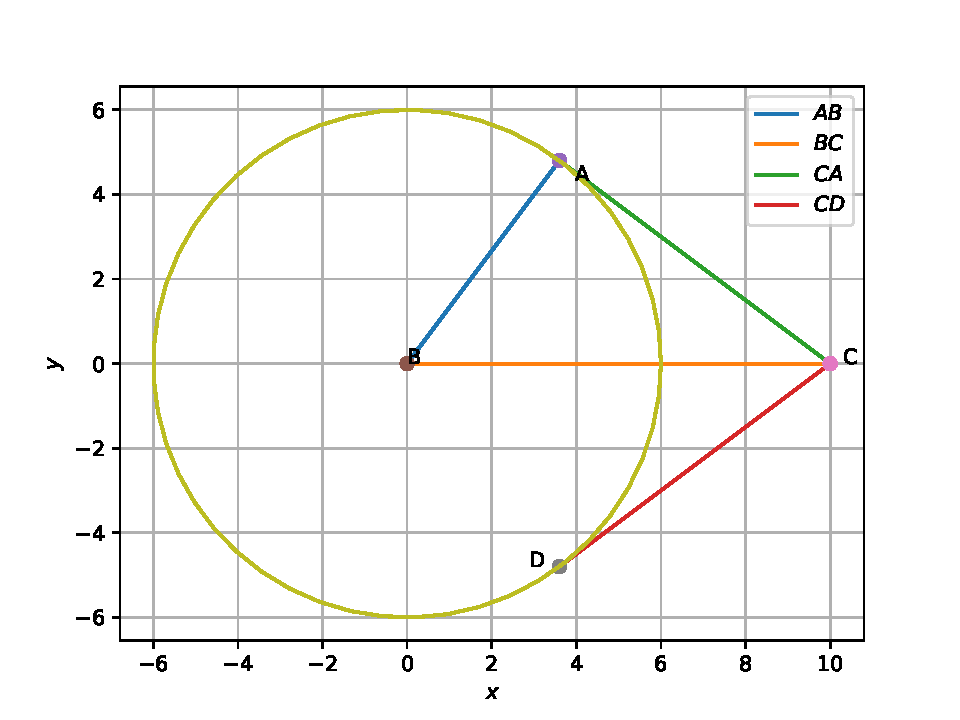
\includegraphics[scale=0.4]{circle.jpg} \\*
If the correct matches are A-p,s and t;B-q and r; C-p and q and D-s then the correct darkening of bubbles will look like the given.
\item z$\neq$ 0 is a complex number\\
\begin{tabular}{llll}
\textbf{Column-I} &   \enspace   &   \textbf{Column-II}\\
(A) $Rez=0$ &   \enspace  &   (p)$Rez^2=0$\\
&&&\\
(B) $Argz=\frac{\pi}{4}$    &   \enspace   & (q)$Imz^2-6$\\
&&&\\
          &\enspace   &   (r)$Imz^2-6$\\
&&&\\
\end{tabular}
\item Match the statements in \textbf{Column-I} with those in \textbf{Column-II}\\
NOTE:Here z takes values in the complex plane and Im z and Re Z denote, respectively,the imaginary part and real part of z
\begin{tabular}{llll}
\textbf{Column-I} &  \enspace   &  \textbf{Column-II}\\
(A) The set of points z satisfying\\
 $\abs {z-iz}=\abs{z+iz} $ is contained in or equal to  &   \enspace   & (p)n ellipse with eccentricity$\frac{4}{5}$\\
&&&\\
(B) The set of all points satisfying \\
$\abs {z+4}+\abs{z-4}=10$ is contained \\
in or equal to   &   \enspace   & (q)the set of points z satisfying  $Imz=0$\\
&&&\\
(C) If $\abs{w}$=2, then the set of points\\
 $z=w-\frac{1}{w}$  &   \enspace  & (r)the set of points z satisfying $\abs{ Im z} \leq 1$\\
&&&\\
(D) If $\abs{ w} =1$, then the set of points\\
    $z=w+\frac{1}{w}$ is contained in or equal to  &   \enspace   & (s) the set of points z satisfying  $Rez\leq 2$\\*
&&&\\
\end{tabular}\\
\clearpage
    \textbf{DIRECTIONS(Q.3)} Following question has matching lists. The codes for the list have choices(a),(b),(c) and (d) out of which ONLY ONE is correct

    \item Let $z_k=cos(\frac{2k\pi}{10})+isin(\frac{2k\pi}{10});k=1,2,3........9$\\*
\begin{tabular}{llll}
\textbf{LIST-I} & \enspace & \textbf{LIST-II}\\&&&\\ 

(P) For each $z_k=$ there exists as \\
$z_j$ such that $z_k,z_j=1$ &   \enspace   &   (1)Trues\\
&&&\\
(Q) There exists a $k\in \{a,2........9\}$ such that\\
 $z_1,z=z_k$ has no solution z in the set of complex numbers    &   \enspace  & (2)False\\
&&&\\
(R) $\frac{\abs{ 1-z_1} 1-z_2...\abs{ 1-z_9}}{10}$ equals   &   \enspace   & (3)1\\    
&&&\\
(S) 1-$\sum_{k=1}^{9}(\frac{2k\pi}{10})$    &   \enspace  & (3)2\\          
&&&\\
\end{tabular}
       \textbf{P}\hspace{5pt}\textbf{Q}\hspace{5pt}\textbf{R}\hspace{5pt}\textbf{S}\\*
    (a) {1}\hspace{5pt}{2}\hspace{5pt}{4}\hspace{5pt}{3}\\*     
    (b) {1}\hspace{5pt}{2}\hspace{5pt}{3}\hspace{5pt}{4}\\*
    (c) {2}\hspace{5pt}{1}\hspace{5pt}{3}\hspace{5pt}{4}\\*
    (d) {2}\hspace{5pt}{1}\hspace{5pt}{4}\hspace{5pt}{3}\\* 
\end{enumerate}
%\end{document}
    
